\documentclass[11pt,a4paper]{report}
\usepackage[utf8]{inputenc}
\usepackage[french]{babel}
\usepackage[T1]{fontenc}
\usepackage{amsmath}
\usepackage{amsfonts}
\usepackage{amssymb}
\usepackage{graphicx}
\usepackage{geometry}
\usepackage{fancyhdr}
\usepackage{chngcntr}
\usepackage{xtab}
\usepackage[hyphens]{url}
\usepackage{longtable}
\usepackage[table]{xcolor}
\usepackage{lscape}
\usepackage{booktabs}
\usepackage{numprint}

\renewcommand{\arraystretch}{1.2}
\definecolor{lightgray}{gray}{0.9}
\definecolor{darkgray}{gray}{0.6}

%----------------------------------------------------------------------------------------
%Commande image tableau de comparaison
%----------------------------------------------------------------------------------------
\newcommand{\ok}{
\includegraphics[width=0.5cm]{check.png}}
\newcommand{\nok}{
\includegraphics[width=0.5cm]{nok.png}}
\newcommand{\unk}{
\includegraphics[width=0.5cm]{unknown.png}}

%----------------------------------------------------------------------------------------
%Tikz
%----------------------------------------------------------------------------------------
\usepackage{tikz}
\usetikzlibrary{shapes.geometric,arrows,matrix}
\tikzstyle{arrow} = [thick,->,>=stealth]
\tikzstyle{header} = [rectangle, minimum height=1.2cm, minimum width=1cm, text width = 2cm, text centered, draw =black,anchor=center] 

%----------------------------------------------------------------------------------------
%Mise en page
%----------------------------------------------------------------------------------------
\geometry{ a4paper,
				   left=20mm,
				   top=25mm,
				   right=15mm,
				   bottom=25mm,
				   headheight=13.6pt} 

%----------------------------------------------------------------------------------------
%Pagination en chiffre romain
%----------------------------------------------------------------------------------------
\pagenumbering{roman}

%----------------------------------------------------------------------------------------
%Figure en chiffre romain
%----------------------------------------------------------------------------------------
\counterwithout{figure}{chapter}
\renewcommand{\thefigure}{\Roman{figure}}

%----------------------------------------------------------------------------------------
%Numerotation des chapitres
%----------------------------------------------------------------------------------------
\makeatletter
\@addtoreset{chapter}{part}
\makeatother
%----------------------------------------------------------------------------------------
% Création du style 
%----------------------------------------------------------------------------------------
\fancypagestyle{EPHEC}{%
  \fancyhf{}% Clear header and footer
  \fancyhead[R]{\thepage}% Custom header
  \renewcommand{\headrulewidth}{0.4pt}
  \renewcommand{\footrulewidth}{0pt}}

%----------------------------------------------------------------------------------------
%Redéfinition du style plain
%----------------------------------------------------------------------------------------
\fancypagestyle{plain}{%
  \fancyhf{}%
  \fancyhead[R]{\thepage}%
  \renewcommand{\headrulewidth}{0.4pt}
  \renewcommand{\footrulewidth}{0pt}}

\pagestyle{EPHEC}

\begin{document}
\begin{titlepage}
\newcommand{\HRule}{\rule{\linewidth}{0.5mm}} % Defines a new command for the horizontal lines, change thickness here

\center % Center everything on the page
 
%----------------------------------------------------------------------------------------
%	HEADING SECTIONS
%----------------------------------------------------------------------------------------

\textsc{\large ÉCOLE PRATIQUE DES HAUTES ETUDES COMMERCIALES}\\[0.5cm] % Name of your university/college

%----------------------------------------------------------------------------------------
%	LOGO SECTION
%----------------------------------------------------------------------------------------


\includegraphics[width=5cm]{ephec.png}\\[0.5cm] % Include a department/university logo - this will require the graphicx package
 
%----------------------------------------------------------------------------------------

\textsc{Avenue du Ciseau, 15}\\ % Minor heading such as course title
\textsc{1348 Louvain-la-Neuve}\\[1.5cm] % Minor heading such as course title

%----------------------------------------------------------------------------------------
%	TITLE SECTION
%----------------------------------------------------------------------------------------

{ \huge \bfseries Installation, configuration et comparaison de solutions professionnelles d'accès à distance}\\[0.4cm] % Title of your document
\HRule \\[0.4cm]
\textsc{\small Travail de fin d'études présenté en vue de l'obtention du diplôme de bachelier en Informatique et Systèmes : finalité Technologie de l'informatique}\\[1.5cm] % Minor heading such as course title
 
%----------------------------------------------------------------------------------------
%	AUTHOR SECTION
%----------------------------------------------------------------------------------------

\begin{minipage}{0.4\textwidth}
\begin{flushleft} \large
\emph{Auteur:}\\
Christian \textsc{JUCKLER} 3TL1 % Your name
\end{flushleft}
\end{minipage}\\

\includegraphics{ephec.png}\\
\begin{minipage}{0.4\textwidth}
\begin{flushleft} \large
\emph{Rapporteur:} \\
Virginie \textsc{Van den Schriek} % Supervisor's Name
\end{flushleft}
\end{minipage}\\[4cm]


%----------------------------------------------------------------------------------------
%	DATE SECTION
%----------------------------------------------------------------------------------------

{\large Année Académique 2014-2015}\\[3cm] % Date, change the \today to a set date if you want to be precise

\vfill % Fill the rest of the page with whitespace

\end{titlepage}
\begin{abstract}
Test
\end{abstract}
\tableofcontents
\listoftables
\addcontentsline{toc}{chapter}{Liste des tableaux}
\listoffigures
\addcontentsline{toc}{chapter}{Liste des figures}
\clearpage
\chapter*{Lexique}
\addcontentsline{toc}{chapter}{Lexique}
Afin de faciliter la lecture, je met à disposition une liste des abréviations utilisées dans ce rapport.

\begin{longtable}{ll}
AAA & Authentication-Authorization-Accounting\\
AD & Active Directory\\
AES & Advanced Encryption Standard\\
AH & Authentication Header\\
ASA & Adaptive Security Appliance\\
ATM & Asynchronous Transfer Mode\\
CA & Certifcate Authority\\
CBC & Cipher Block Chaining\\
CHAP & Challenge-handshake Authentication Protocol\\
CRM & Customer Relationship Manager\\
DES & Data Encryption Standard\\
DFS & Distributed File System\\
DLCI & Data Link Connection Identifier\\
DMZ & Demilitarized Zone\\
ECDHE & Elliptic Curve Diffie-Hellman Exchange\\
ESP & Encapsulating Security Payload\\
ETTD & Equipement terminal de transmission de données\\
GPO & Group Policy Object\\
HDR & Header\\
IETF & Internet Engineering Task Force\\
IKE & Internet Key Exchange\\
IP & Internet Protocol\\
IPSec & Internet Protocol Security\\
IVC & Integrity Check Value\\
KE & Key Exchange\\
MAC & Message Authentication Code\\
OU & Organizational Unit\\
OWA & Outlook Web App\\
PAP & Password Authentication Protocol\\
PPP & Pont-to-Point Protocol\\
PVC & Permanent Virtual Circuit\\
SA & Security Association\\
SHA & Secure Hash Algorithm\\
SSL & Secure Sockets Layer\\
SVC & Switched Virtual Circuit\\
TLS & Transport Layer Security\\
UDP & User Datagram Protocol\\
VPN & Virtual Private Network\\
WAN & World Area Network\\
\end{longtable}
\chapter*{Introduction}
\addcontentsline{toc}{chapter}{Introduction}
Un VPN est un réseau privé construit sur une infrastructure publique. 
Il permet à une entreprise de connecter de façon sécurisée des sites et/ou des utilisateurs distants.
Ce n'est pas la seule utilité des VPN. 
Mais pour ce travail, je ne m'intéresse qu'à l'utilisation des VPN en entreprise.
Auparavant, les tunnels VPN étaient construits sur des réseaux privés que les entreprises louaient auprès des fournisseurs de télécommunication.
De nos jours, l'infrastructure publique utilisée est le réseau Internet pour des raisons financières et de disponibilité.

Les données transitant par l'Internet peuvent être interceptées.
En cas d'interception, les données sont lisibles par le pirate, à moins que les données soient chiffrées avec un protocole de chiffrement robuste.
La sécurisation des VPN est un enjeu essentiel pour éviter la fuite d'information sensible.

L'utilisation de VPN sécurisé est un élément important des entreprises pour la productivité des utilisateurs distants. 
Un utilisateur distant ne se résume plus à un commercial visitant des sièges en divers lieux.
On y trouve tous les types d'employées. Par exemple, le télé-travailleur qui veut échapper aux embouteillages sur la route; le consultant informatique qui doit faire une intervention chez un client.

Les philosophies de sécurisation étant différentes d'une solution à une autre, un comparatif des solutions professionnelles ... 
\pagenumbering{arabic}
\part{La problématique des accès distants en entreprise}
\chapter{Les besoins habituels}
\chapter{Les besoins spécifiques}
\chapter{La situation actuelle}
\begin{figure}

\includegraphics{ephec.png}
\caption{Test figure}
\end{figure}
\chapter{Méthodologie et objectifs}
\part{Technologies d'accès distant}
\chapter{Description des technologies}
Dans ce chapitre, je présente les technologies d'accès distants.
Dans un premier temps, je commence par expliquer les notions des VPN et de tunnel VPN. 
De plus, j'y expose les protocoles de tunneling et de chiffrement.
Par la suite, je détaille les protocoles qui peuvent former des tunnels VPN sécurisés. 
Finalement, je passe en revue les solutions propriétaires et celles des fournisseurs d'accès pour les accès distants.

\section{Virtual Private Network - VPN}
Le terme VPN est un acronyme pour « Virtual Private Network ».
Un VPN est par définition un réseau virtuel qui transfère des données privées en créant un tunnel à travers un réseau public.

Historiquement, les VPN étaient construits sur des lignes louées, mais le coût de ces infrastructures était trop important.
Maintenant, les VPN sont basés sur l'Internet dont l'avantage principal est son faible coût.
Mais en utilisant l'Internet, les données privées deviennent accessibles à tout le monde. 
Il a donc été nécessaire de fournir des protocoles permettant d'assurer la confidentialité et l'intégrité des données à travers le réseau public. 

Un tunnel VPN est monté entre deux passerelles VPN ou entre deux hôtes. 
Les deux équipements sont d'un point de vue logique connectées directement l'une à l'autre. 
Le tunnel permet d'envoyer des données du réseau privé à travers le réseau public.
Il encapsule les données dans un protocole compris par les deux extrémités. 
L'émetteur encapsule les données et le destinataire récupère les données. 
En plus de l'encapsulation des données, les tunnels VPN réalisent du chiffrement. 

\subsection{Les types de VPN}
Il existe deux grands types de VPN : les VPN site-à-site et les VPN client-à-site ou VPN "remote access".

\subsubsection{Les VPN site-à-site} 
Ils sont utilisés pour connecter des sites entre eux. 
Le tunnel est monté entre deux passerelles VPN dont les configurations sont connues. 
Le réseau Internet opère comme une liaison WAN entre les sites. 
Les employées peuvent échanger des informations entre les différents sites comme s'ils sont connectés sur le site distant. 
Dans ce cas-ci, nous utilisons principalement des tunnels VPN IPsec. 

\subsubsection{Les VPN client-à-site} 
Ils sont généralement utilisés par des travailleurs pour accéder aux ressources de l'entreprise depuis des emplacements non fiables.  
L'utilisateur se connecte via son ordinateur ou son smartphone à la passerelle VPN de son entreprise.  
Dans ce cas, la configuration n'est pas connue, car selon la localisation de l'utilisateur, les paramètres de connexion changent.  
Il est souvent nécessaire d'installer sur l'appareil mobile un client VPN. 
Nous utilisons majoritairement des tunnels VPN SSL pour leur simplicité de configuration. 
Bien qu'il soit possible de créer des tunnels de ce type avec IPSec.
L'utilisation de SSL est soumise à controverse depuis la découvert de \textit{Hearthbleed}.

Avant de présenter les protocoles IPSec, SSL et TLS, intéressons-nous au protocole de tunneling.
\subsection{Les protocoles de tunneling de couche 2}
Avant de créer le tunnel, ces protocoles se mettent d'accord sur des paramètres de session, comme le protocole de chiffrement.
Une fois les paramètres acceptés par les deux extrémités, le tunnel est monté.
Les données sont envoyées via ce tunnel entre les deux extrémités.
Il est possible de transmettre des données issues de protocole non-routable à travers le réseau public. 
Les données sont encapsulés dans un autre protocole qui est routable.

Par exemple, le protocole AppleTalk n'est pas supporté par l'Internet, mais grâce au tunnel, nous encapsulons le paquet AppleTalk dans un paquet IP. 
Ce paquet est envoyé sur l'Internet qui va le transmettre au destinataire.
Ce dernier désencapsule le paquet IP et récupère le paquet AppleTalk. 

Il est nécessaire que les deux extrémités du tunnel comprennent le protocole encapsulé.
Sinon, la destination ne saura pas capable de traiter le paquet encapsulé. 

\subsubsection{Point-to-Point Tunneling Protocol - PPTP}
C'est un protocole propriétaire de Microsoft.
Il est implémenté depuis Windows 2000 dans toutes les machines Windows et il existe des clients PPTP pour Linux et OS X.
Sa configuration est simple, mais la sécurité qu'il propose n'est pas exempt de tout reproche.

Ce protocole encapsule des frames PPP\footnote{Point-to-Point Protocol} dans un tunnel IP.
Il fonctionne en quatre phases dont une est optionnelle : Link Establishment Phase, Authentication Phase, Callback Control Phase, Network Control Phase.
\begin{enumerate}
	\item La phase une sert à établir, maintenir et terminer la connexion physique entre les deux hôtes. C'est aussi à ce moment que les protocoles d'authentification sont choisis.
	\item Le client PPTP est authentifié en utilisant le protocole PPP. L'authentification peut se faire en claire ou en utilisant des protocoles comme PAP et CHAP. 
	\item La phase trois est optionnel et elle permet une sécurité accrue. Elle déconnecte le client et le serveur. Ensuite, le serveur rappelle le client. 
	\item La dernière phase sert à négocier et implémenter les protocoles de compression et de chiffrement.
\end{enumerate}
\subsubsection{Layer 2 Tunneling Protocol - L2TP}
Ce protocole a été normalisé en utilisant les avantages des protocoles PPTP et L2F de Cisco\footnote{Layer 2 Forwarding}. 
Mais il ne permet toujours pas la confidentialité du trafic. 
Il est possible de faire de l'authentification et du chiffrement avec les paquets PPP, mais la connexion reste vulnérable au niveau de la couche transport. 
Il est donc intéressant d'associer L2TP avec un autre protocole de sécurité comme IPSec.

PPTP  et L2TP ne possèdent pas un niveau de sécurité élevé pour être utilisé comme tunnel VPN à travers Internet.
Ils sont le plus souvent remplacer par des tunnels IPSec ou SSL, qui possèdent un meilleur niveau de sécurité.
\section{Internet Protocol Security - IPSec}
IPsec est un ensemble de protocole visant à sécuriser les données au niveau de la couche réseau. 
Il est composé de trois protocoles : AH (\textit{Authentication Header}), ESP (\textit{Encapsulating Security Payload}) et IKE (\textit{Internet Key Exchange}).
IKE est utilisé lors de la négociation des paramètres du tunnel VPN. 
Les deux autres protocoles fournissent la sécurité des données en les encapsulant au sein du tunnel VPN. 

\subsection{Les protocoles AH et ESP}
Le protocole AH permet uniquement l'authentification. 
L'authentification se fait à l'aide d'un algorithme MAC \footnote{Message Authentication Code} tel que MD5 ou SHA-1.
Cette algorithme prend en input des éléments de l'en-tête IP et calcule un IVC \footnote{Integrity Check Value}.
L'IVC est ajouté dans l'en-tête AH et ce dernier est ajouté au paquet IP.

Le protocole ESP permet l'authentification et le chiffrement des données.

Un schéma des paquets formés est disponible sur la Fig.\ref{fig:ipsecHead} p.\pageref{fig:ipsecHead}.

\begin{figure}
	\centering
	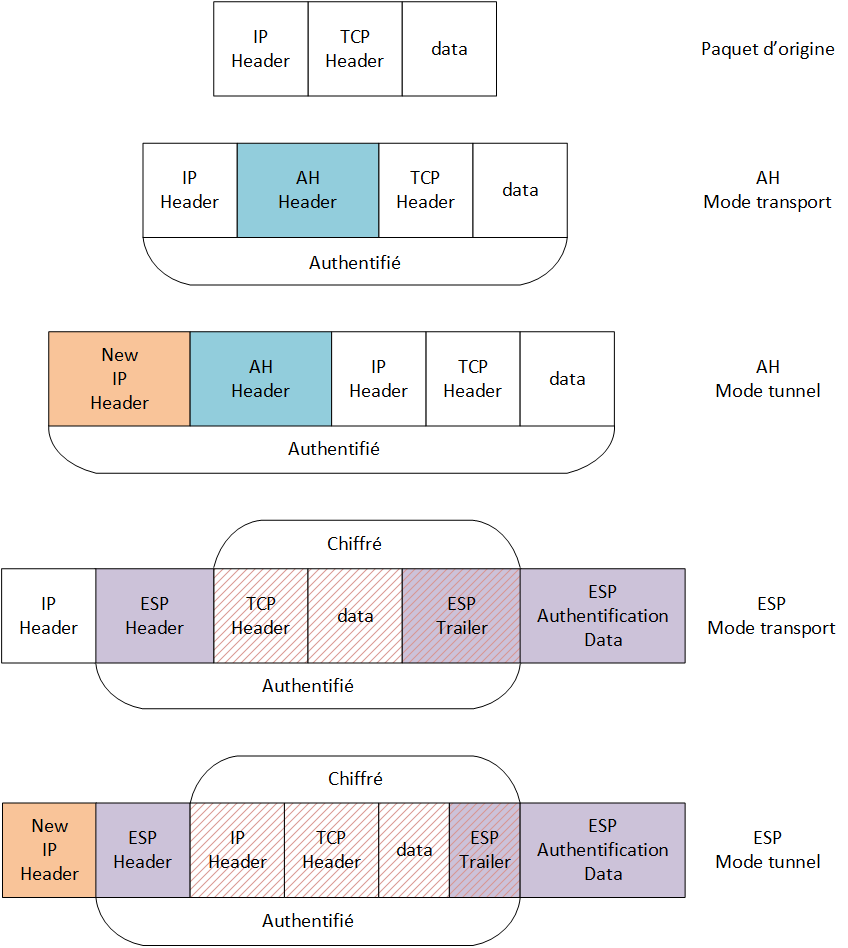
\includegraphics[width=16cm]{techno/IPSec-AH-ESP}
	\caption{Format des paquets IPSec}
	\label{fig:ipsecHead}
\end{figure}

\subsection{Les modes transport et tunnel}
Le mode transport est utilisé pour des connexions bouts-à-bouts entre deux hôtes.

Le mode tunnel est préféré lorsque l'un ou les deux hôtes de la communication sont des passerelles VPN.

\subsection{IPSec et le NAT}
Comme vu précédemment (Fig.\ref{fig:ipsecHead} p.\pageref{fig:ipsecHead}), IPSec protège les en-têtes des paquets IP.
Pour le protocole AH, le moindre changement au niveau des adresses IP provoque une erreur dans l'IVC vu que l'authentification s'applique au paquet entier.
Pour le protocole ESP, l'en-tête ESP est un paquet de la couche réseau. Il ne possède pas d'information sur les ports, qui sont des éléments de la couche transport.
Il n'est pas possible d'associer un port unique pour cette communication.

Pour palier à ces problèmes, une solution est d'encapsuler les paquets IPSec dans un autre paquet.
Ainsi le NAT-T (NAT-Traversal) encapsule les paquets IPSec dans un paquet UDP avec le port 4500 (par défaut).
Ainsi, c'est l'en-tête UDP qui sera modifier lors du transfert entre les deux hôtes et le paquet IPSec ne sera pas modifié.

\subsection{Security association}
Quand nous parlons de monter un tunnel, en réalité, nous synchronisons un état partagé entre les terminaisons du tunnel. 
Cet état partagé se nomme une SA (\textit{security association}) en IPSec. 
Une SA contient l'algorithme de chiffrement utilisé et les clés utilisées, l'algorithme d'authentification, un numéro d'identifiant, le \textit{security parameter index} (SPI), … 
Plus d'autres paramètres qui servent à maintenir les tunnels VPN. 
Les SA peuvent être créées manuellement ou gérées par l'IKE. 
Chaque terminaison possède deux SA, une pour le trafic entrant et une pour le trafic sortant. 
De plus, chaque paire est liée à un protocole. 
Les SA se caractérisent par un triplet formé du SPI, de l'adresse de destination et du protocole. 
Les SA sont stockées dans une SAD (\textit{security association database}). 
Cette SAD est utilisée pour déterminer quel protocole est utilisé pour les paquets sortants et pour fournir les paramètres pour déchiffrer et/ou authentifier les paquets entrants. 
Il est possible de combiner les SA pour créer des tunnels VPN complexe. 

Les SA sont des éléments simples, c'est-à-dire qu'elles traitent tous les paquets de la même manière. 
Pour un réglage plus fin, IPSec utilise des policies. 
Ces policies se basent sur les champs suivants des en-têtes du paquet.
\begin{itemize}
\item L'adresse de destination
\item L'adresse source
\item Le protocole de la couche transport
\item Le port source
\item Le port de destination
\end{itemize}
Elles servent à déterminer quels paquets à émettre sur quel tunnel, à dropper les paquets ne correspondant à aucune des règles décrites dans les policies. 
De la même manière que les SA, les policies sont stockées dans une SPD (\textit{security policy database}). 
Le fonctionnement est similaire, pour chaque paquet entrant ou sortant, le système consulte la SPD pour déterminer les règles à appliquer au paquet. Si une règle est trouvée, le système cherche après la SA correspondante.

\subsection{Le protocole IKE}
IKE a un seul objectif : procéder à des échanges de clé Diffie-Hellman pour sécuriser un tunnel VPN. 
Il négocie le chiffrement, l'authentification nécessaire au tunnel, qui satisfont les policies. 

IKE dérive du \textit{Internet Security Association and Key Management} Protocol (ISAKMP). 
ISAKMP est un framework qui fournit des outils pour la sécurisation des échanges et l'échange de clé. 
De plus, IKE utilise différents mode du protocole OAKLEY.
Il établit une SA en deux phases et il possède cinq modes d'échange, dont trois découlent d'ISAKMP.
Les deux derniers modes ne sont utilisés que lors de la phase deux.

\subsubsection{La phase 1 d'IKE}
La phase 1 crée un canal sécurisé entre les terminaux du tunnel pour déterminer les SA. 
Le canal sécurisé est créé après l'authentification des terminaux. 
Les SA de la phase 1 sont bidirectionnelles, c'est-à-dire qu'une SA sécurise le trafic entrant et sortant. 
Pour l'échange des SA de la phase 1, IKE possède deux modes d'échanges : 
\begin{itemize}
	\item Main mode
	\item Agressive mode
\end{itemize}

Le mode \textit{"main"} d'IKE travaille en trois étapes (voir Fig.\ref{fig:ipsmain} p.\pageref{fig:ipsmain}).
Il est utilisé lorsque les terminaux possèdent des adresses IP statiques. 
\begin{figure}[ht]
\centering
\begin{tikzpicture}
	\draw[-,ultra thick] (0,7) node [above] {Initiator} -- (0,0) ;
	\draw[-,ultra thick] (7,7) node [above] {Responder}-- (7,0);
	\draw[arrow] (0,6) -- (7,6) node [midway,above] {HDR - SA};
	\draw[arrow] (7,5) -- (0,5) node [midway,above] {HDR - SA};
	\draw[arrow] (0,4) -- (7,4) node [midway,above] {HDR - KE - NONCE$_i$};
	\draw[arrow] (7,3) -- (0,3) node [midway,above] {HDR - KE - NONCE$_r$};
	\draw[arrow] (0,2) -- (7,2) node [midway,above] {HDR - ID$_i$ - \textit{AUTH}};
	\draw[arrow] (7,1) -- (0,1) node [midway,above] {HDR - ID$_r$ - \textit{AUTH}};
\end{tikzpicture}
\caption{IPsec : mode "main"}
\label{fig:ipsmain}
\end{figure}
Premièrement, l'initiateur envoie un message contenant une liste des méthodes de sécurisation qu'il utilise. 
Le receveur choisit dans la liste reçue la méthode correspondant à ses policies et envoie sa décision à l'initiateur. 
Ensuite, ce dernier envoie sa clé privée pour créer le secret partagé de l'algorithme de Diffie-Hellman. 
Le receveur fait de même. Ils sont donc capables tous les deux de créer les clés. 
Les clés dépendent des méthodes d'authentification choisies. 
Finalement, l'initiateur envoie son identité et des informations sur l'authentification. 
Ces messages sont chiffrés et masquent donc l'identité des terminaux. 
L'échange se fait en six messages.

À la fin de ce mode, les terminaux sont d'accord sur les algorithmes de chiffrement et de confidentialité des données. 
Ils possèdent également les clés pour les algorithmes sélectionnés. 

Le mode \textit{"agressive"} fait le même travail de façon plus rapide, il n'utilise que trois messages (voir Fig.\ref{fig:ipsagg} p.\pageref{fig:ipsagg}).
Il est utilisé lorsque l'un des deux terminaux de la connexion possède une adresse IP dynamique.
\begin{figure}[ht]
\centering
\begin{tikzpicture}
	\draw[-,ultra thick] (0,4) node [above] {Initiator} -- (0,0) ;
	\draw[-,ultra thick] (8,4) node [above] {Responder}-- (8,0);
	\draw[arrow] (0,3) -- (8,3) node [midway,above] {HDR - SA - KE - NONCE$_i$ - ID$_i$};
	\draw[arrow] (8,2) -- (0,2) node [midway,above] {HDR - SA - KE - NONCE$_r$ - ID$_r$ - \textit{AUTH}};
	\draw[arrow] (0,1) -- (8,1) node [midway,above] {HDR - \textit{AUTH}};
\end{tikzpicture}
\caption{IPsec : mode "agressive"}
\label{fig:ipsagg}
\end{figure} 
Lors du premier envoi, l'initiateur émet la liste des méthodes de sécurisation, son identité et sa clé. 
Le receveur répond par son choix de sécurisation, sa clé, son identité et ses identifiants. 
Finalement l'initiateur s'authentifie auprès du receveur. 
Ce dernier message peut être chiffré.

Pour l'authentification d'un terminal, il existe trois méthodes : 
\begin{itemize}
	\item Kerberos
	\item Certificats	
	\item Public Key Infrastructure (PKI)
\end{itemize}

\paragraph{Kerberos}
Kerberos est un protocole réseau d'authentification par clé chiffré.
Il fournit une forte authentification à condition que tous les services utilisent Kerberos.
Il a été conçue par le MIT\footnote{Massachusetts Institute of Technology} à la fin des années 80.
Actuellement, il est recommandé d'utiliser la version 5, qui corrige des bugs critiques de la version 4.
Kerberos est disponible sur la plupart des systèmes d'exploitation actuels.
Une version gratuite est disponible sur le site du MIT, et il existe des versions commerciales.

Pour qu'un hôte puisse se connecter à un service, le système vérifie son identité, et le cas échéant accepte ou refuse la connexion.
Ce système repose sur deux serveurs sécurisés, un serveur d'authentification (AS\footnote{Authentication Server}) et un serveur d'octroi de ticket (TGS\footnote{Ticket-Granting Server}).
Ils forment dans la terminologie Kerberos un centre de distribution de ticket ou KDC\footnote{Key Distribution Center} en anglais.
De plus, Kerberos utilise des clés chiffrées pour toutes les communications.

\paragraph{Certificat}
Un certificat n'est rien de plus qu'une clé publique accompagnée d'un identifiant dont l'ensemble des informations sont signées par un tiers de confiance.
Ce tiers est ce que l'on appelle une autorité certificative (CA). 
Elle est reconnue au niveau mondiale.
Un utilisateur envoie sa clé publique au CA et reçoit en retour, après vérification, son certificat signé par la CA.

\paragraph{PKI}
Une PKI est un ensemble de composants et de processus informatiques, humains et techniques dont le but est de gérer la distribution et la vie des certificats.

\subsubsection{La phase 2 d'IKE}
Une fois la SA établie, les terminaux peuvent l'utiliser pour négocier les SA de phase 2. 
La phase 2 est un échange en Quick mode. 
L'échange se fait en trois messages. 
Lors de l'échange, il est possible de négocier plusieurs SA en même temps. 
\section{Secure sockets layer - SSL}
Netscape a lancé SSL 1 en 1994, dans le but de sécuriser des transactions réalisées avec leur navigateur. 
Dans la même année, SSL 2 était déjà en route. 
Mais le protocole montrait déjà des problèmes de sécurité.
Fin 1995, SSL 3 était lancé. 
Il s'agissait d'une version complètement récrite de SSL, qui introduisait de nouvelles fonctionnalités issues de PCT\footnote{Microsoft's \textit{Private Communications Technology}}.
Bien que les machines actuelles intègrent SSL 3, elles essaient d'abord de négocier une connexion en SSL 2.

Dans un effort de standardisation de SSL, l'IETF a lancé le protocole TLS\footnote{Transport Layer Security}.
Il se base principalement sur SSL 3 bien qu'il ne soit pas compatible avec ce dernier.

SSL utilise des suites de chiffrement. Ces suites se composent de trois fonctions de chiffrement : la méthode d'échange de clé, l'algorithme de chiffrement et une méthode de hachage. 
Il existe un large ensemble de suite, les client ont donc un mécanisme pour signaler les suites qu'ils gèrent et qu'ils utilisent. 

OpenSSL est l'implémentation la plus courante de SSL. 
Cette implémentation possède un interface en ligne de commande, qui permet de générer des clés RSA, signer des certificats, calculer des valeurs de hash, ...

\subsection{Le protocole SSL}
SSL est un protocole de la couche transport, il utilise donc les protocoles de cette couche pour le transfert des données. 
Pour éviter des problèmes lors de la transmission des données, SSL utilise le protocole TCP.

De manière analogue à TCP, une session SSL se divise en trois phase (voir Fig.\ref{fig:ssl} p.\pageref{fig:ssl}) : 
\begin{enumerate}
	\item \'Etablissement de la connexion
	\item Transfert des données
	\item Clôture de la connexion.
\end{enumerate}
\begin{figure}[ht]
\centering
\begin{tikzpicture}
	\draw[-,ultra thick] (0,10.8) node [above] {Client} -- (0,0) ;
	\draw[-,ultra thick] (6,10.8) node [above] {Serveur}-- (6,0);
	\draw[arrow] (0,10) -- (6,10) node [midway,above] {Handshake : ClientHello};
	\draw[arrow] (6,9) -- (0,9) node [midway,above] {Handshake : ServerHello};
	\draw[arrow] (6,8.4) -- (0,8.4) node [midway,above] {Handshake : Certificate};
	\draw[arrow] (6,7.8) -- (0,7.8) node [sloped, midway,above] {Handshake : ServerHelloDone};
	\draw[arrow] (0,6.8) -- (6,6.8) node [midway,above] {Handshake : KeyExchange};
	\draw[arrow] (0,6.2) -- (6,6.2) node [midway,above] {ChangeCipherSpec};
	\draw[arrow] (0,5.6) -- (6,5.6) node [midway,above] {Handshake : Finished};
	\draw[arrow] (6,4.6) -- (0,4.6) node [midway,above] {ChangeCipherSpec};
	\draw[arrow] (6,4) -- (0,4) node [midway,above] {Handshake : Finished};
	\draw[arrow] (0,2.6) -- (6,2.6);
	\draw[arrow] (6,2) -- (0,2) node [midway,above] {Application Data};
	\draw[arrow] (0,0.8) -- (6,0.8);
	\draw[arrow] (6,0.2) -- (0,0.2) node [midway,above] {Alert Close Notify};
\end{tikzpicture}
\caption{Session SSL}
\label{fig:ssl}
\end{figure}
La session commence par le \textit{triple handshake}. 
Le client envoie un message ClientHello, qui indique la version de SSL supportée, la liste des suites de chiffrement et les algorithmes de compression. 
La version de SSL est signalée par deux champs dans l'en-tête : version mineur et version majeure. 
SSL3 a une version majeure de 3 et une version mineure de 0, et TLS a un version majeure de 3 et une version mineure de 1. 

Le serveur répond par trois messages.
\begin{enumerate}
	\item Le message \textit{ServerHello} indique au client la suite de chiffrement et l'algorithme de compression à utiliser.
	\item Le certificat du serveur permet au client de vérifier l'identité du serveur et contient la clé publique du serveur. Cette clé va servir à générer les différents clés pour la session.
	\item Le message \textit{ServerHelloDone} précise la fin de la séquence \textit{Hello}.
\end{enumerate}
Suite à ces trois messages, le client donne au serveur des inputs pour la génération des clés (\textit{ClientKeyExchange}), signal au serveur qu'il utilise les nouvelles clés pour le chiffrement et l'authentification (\textit{ChangeCipherSpec}) et qu'il a fini le handshake (\textit{Finished}).
 Le serveur répond avec son message \textit{ChangeCipherSpec} et son \textit{Finished}.
 
 Le client et le serveur sont capables de s'échanger des données de façon sécurisé. 
 
 Finalement, la session est clôturée.
\section{Secure Shell - SSH}
SSH a pour objectif de créer une connexion sécurisée.
De la même manière que SSL, SSH est un protocole de la couche applicative et utilise TCP.
Par contre les applications ne doivent pas forcément intégrer SSH pour être utilisées via SSH.

SSH est principalement utilisé pour remplacer \texttt{telnet}, mais il est également possible de faire du VPN.
En effet, SSH fournit de l'authentification et du chiffrement pour les communications entres les machines.

Les tunnels VPN SSH sont peu utilisés, car ils manquent de performance.
Mais ils sont simple à mettre en place.
\section{Secure Socket Tunneling Protocol - SSTP}
SSTP est utilisé pour transporter du trafic PPP/L2TP via du SSL3.
Son avantage réside dans le fait qu'il peut passer à travers les NAT, les proxys et les firewalls. 
\section{HTTP over TLS/SSL - HTTPS}
Il s'agit rien de plus qu'une connexion HTTP chiffrée par SSL ou TLS.
Il fournit une authentification pour les serveurs Web et un chiffrement bidirectionnel pour les communications entre le navigateur Web et le serveur Web.

La confiance envers un site Web est liée à un certificat. 
Ce dernier doit provenir d'une autorité certificative reconnue au niveau mondiale. 
\section{Propriétaires}

\section{Fournisseurs d'accès}

\chapter{Comparaison théorique}
\chapter{Architecture}
\part{Comparaison des solutions commerciales}
\chapter{Choix des solutions}
Le choix des solutions testées s'est fait sur base des leaders commerciaux.
Cisco et Juniper sont des fabricants de matériel réseau (switch, routeur, firewall, ...).
Microsoft est le leader commercial dans les systèmes d'exploitation.

L'utilisation d'un environnement Windows était inévitable, car les systèmes d'exploitation Windows occupent presque 80\% des parts de marché.
De plus, mon expérience est plus grande dans l'environnement Windows, surtout pour la partie Active Directory.
Il existe des solutions similaires chez Unix et Apple, mais par manque de connaissances de ces produits, il m'a semblé plus évident de construire un environnement Windows dans le cadre de ce TFE.
La solution DirectAccess est assez récente, c'était une bonne opportunité de la tester et de la découvrir.

En plus de fournir du matériel hardware, Cisco et Juniper possèdent des systèmes d'exploitation complet pour la gestion des firewalls et des passerelles.
Chaque fabricant possède sa propre philosophie.
Ainsi Juniper propose une passerelle dédiée au accès distant.
Par contre Cisco fonctionne avec du tout-en-un, la passerelle est intégrée au firewall.
\chapter{Installation et configuration des solutions}
\section{Solution Juniper/Pulse}
La solution de Juniper se base sur l'utilisation d'une passerelle SSL.
Cette passerelle gère les connexions entrantes et attribue, aux connexions autorisées, l'accès aux ressources.
La passerelle utilisée est une SA 2500 tournant sous Pulse Connect Secure 8.1R1.1.
Les clients distants peuvent se connecter soit via le portail Web, soit via le client Pulse Secure.

Le client Pulse Secure est fourni par la passerelle.
Cette dernière peut distribuer le software à tous les utilisateurs authentifiés automatiquement ou en le téléchargeant via le portail Web.

\subsection{Schéma de l'infrastructure}
Comme la passerelle est accessible depuis l'extérieur, elle ne possède pas le même niveau de confiance que le LAN.
Elle est donc placée dans une DMZ.
%\begin{figure}[ht]
%	\centering
%	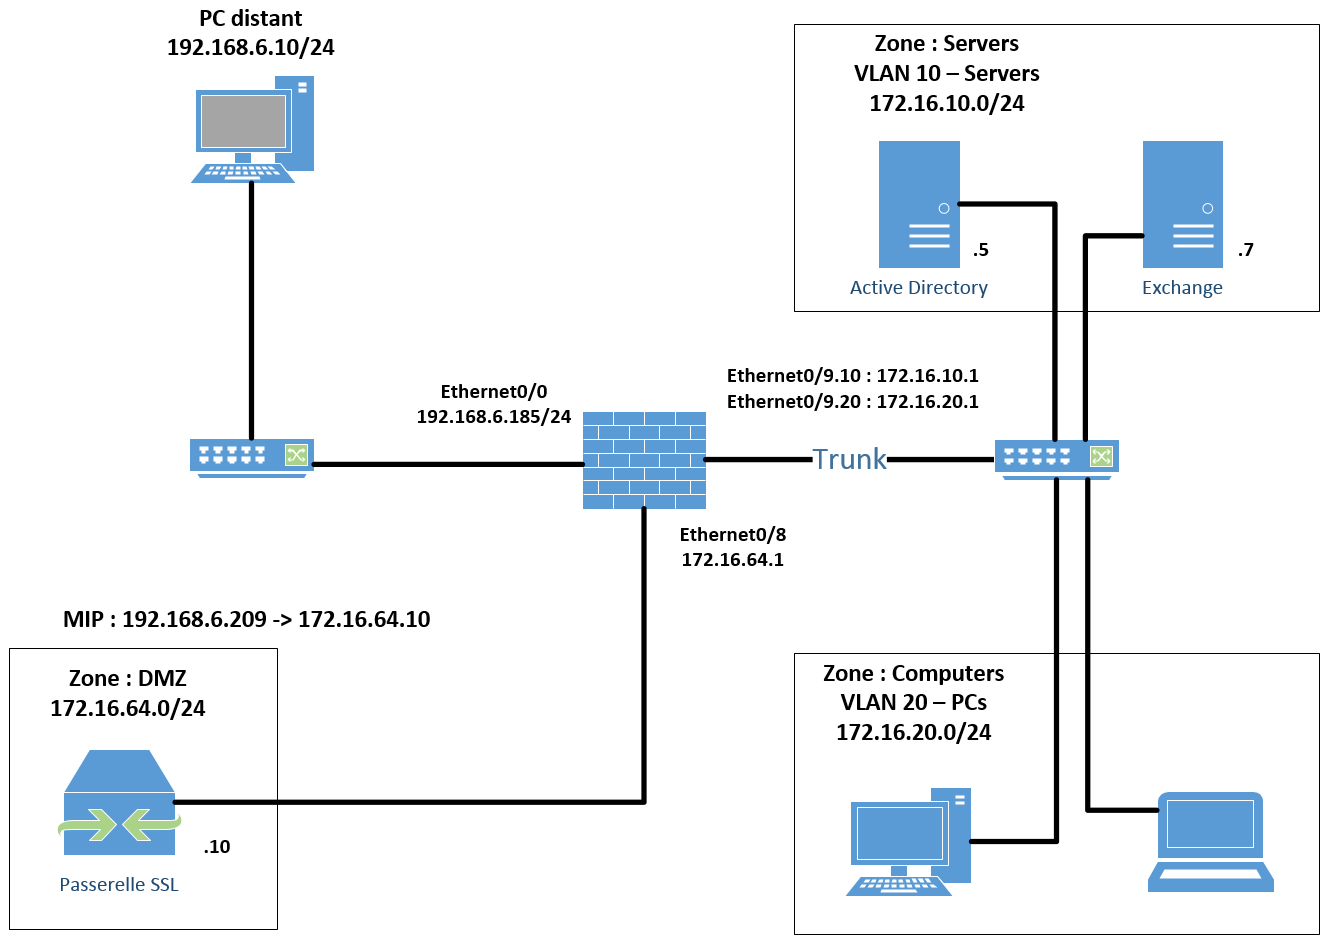
\includegraphics[width=16cm]{juniper/schema.png}
%	\caption{Adressage des interfaces}
%	\label{fig:schemaJuniper}
%\end{figure}

Le firewall sert de routeur entre le réseau du labo (externe) et le réseau de test (interne).
Il gère aussi les \textit{policies}, c'est-à-dire les règles entre les zones de sécurité établies dans la configuration.
Dans mon réseau de test, j'ai créé deux zones en plus de celles pré-définies : la zone "Computers" et "Servers".

Pour l'adressage (Fig.\ref{fig:ifJuniper} p.\pageref{fig:ifJuniper}), ma zone \textit{Untrust} est le labo. 
L'interface associé possède l'adresse 192.168.6.185.
Les autres zones font parties du réseau de test et possèdent une adresse dans le réseau 172.16.0.0/16.
J'utilise les VLAN 10 et 20 pour différencier le trafic des ordinateurs et des serveurs sur le même interface.
L'utilisation de deux zones distinctes est une bonne pratique avec Juniper. 
Il est plus claire de créer des \textit{policies} entre des zones, que de créer des ACL sur les interfaces.
\begin{figure}[ht]
	\centering
	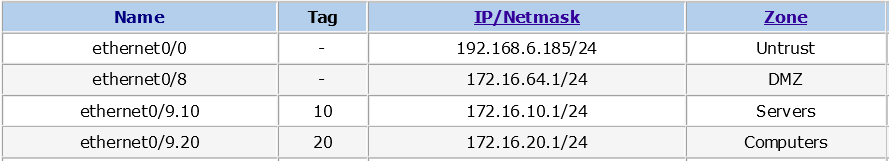
\includegraphics[width=16cm]{juniper/interfaces.png}
	\caption{Adressage des interfaces}
	\label{fig:ifJuniper}
\end{figure}

Pour autoriser l'accès à la passerelle, l'utilisation d'un mappage est indispensable.
On a mappé l'adresse externe (192.168.6.209) avec l'adresse de la passerelle dans la DMZ (172.16.64.10).
Le mappage ne suffit pas, il faut aussi autoriser le trafic entre la zone \textit{Untrust} et la DMZ (Fig.\ref{fig:polUnDMZ} p.\pageref{fig:polUnDMZ}).
En suivant les règles de bonnes pratiques, j'autorise uniquement le trafic HTTPS et ESP entre un client en remote-access et la passerelle et je bloque tous les autres trafics.
\begin{figure}[ht]
	\centering
	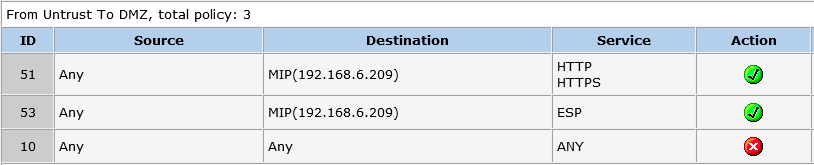
\includegraphics[width=16cm]{juniper/Policy-Untrust-DMZ.png}
	\caption{Policies entre la zone Untrust et la DMZ}
	\label{fig:polUnDMZ}
\end{figure}

\subsection{Configuration de la passerelle  SSL}
\subsubsection{\textit{Realm} et rôles}
Pour commencer, on définit le \textit{realm} d'authentification.
Il existe plusieurs possibilités, j'ai choisi d'utiliser une authentification simple via l'Active Directory.
Ce mode d'authentification est fiable, mais pour une sécurité renforcée, il est intéressant de passer à une double authentification.
La double authentification s'active en cochant l'option dans la configuration du \textit{realm} (voir Fig.\ref{fig:confRealm} p.\pageref{fig:confRealm}).
\begin{figure}[ht]
	\centering
	\includegraphics[width=16cm]{juniper/Authserv.png}
	\caption{Configuration du \textit{realm} d'authentification}
	\label{fig:confRealm}
\end{figure}

À chaque realm, on mappe l'utilisateur à un rôle.
Dans mon cas, mes utilisateurs appartiennent soit au rôle "It Tech", soit au rôle "All Employee".
Cette attribution dépend du groupe Active Directory auquel appartient l'utilisateur (voir Fig.\ref{fig:mapRoles} p.\pageref{fig:mapRoles}). 
\begin{figure}[ht]
	\centering
	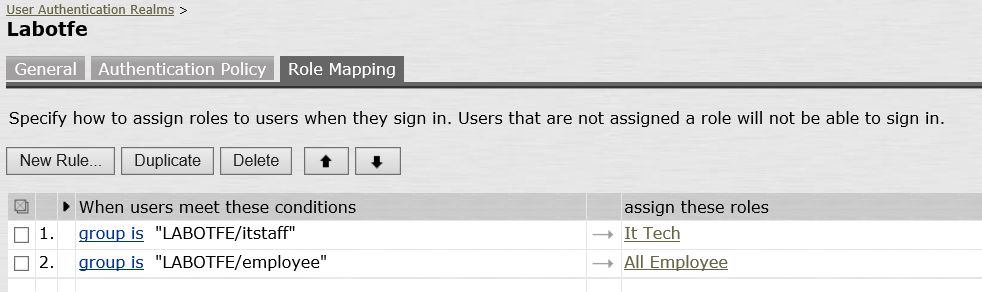
\includegraphics[width=16cm]{juniper/Rolemapping.png}
	\caption{Mappage des rôles dans le realm}
	\label{fig:mapRoles}
\end{figure}

À ces deux rôles, j'ai associé des ressources différentes (voir Fig.\ref{fig:resRoles} p.\pageref{fig:resRoles}).
\begin{figure}[ht]
	\centering
	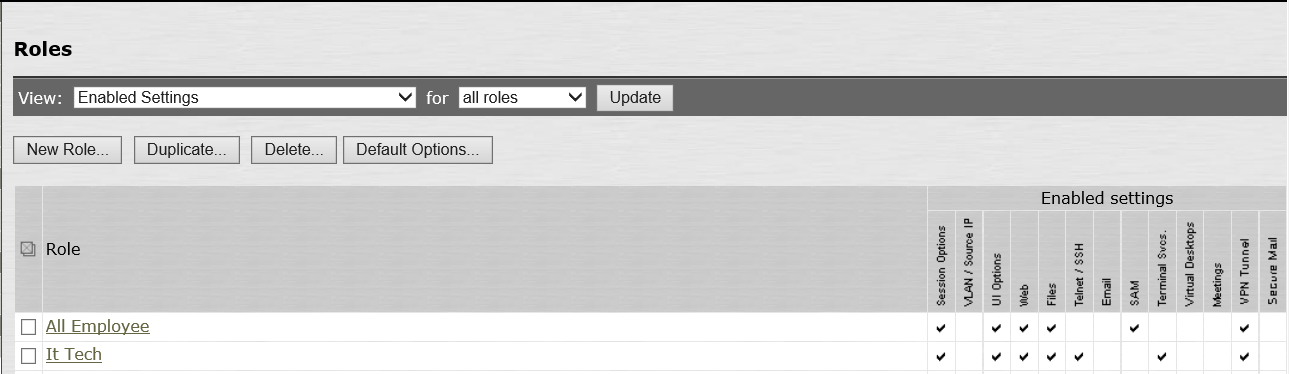
\includegraphics[width=16cm]{juniper/UserRoles.png}
	\caption{Ressources associées aux rôles}
	\label{fig:resRoles}
\end{figure}

\subsubsection{VPN - Portail Web}
Le portail Web se configure en créant une "Sign-in Pages".
Les utilisateurs distants y accèdent via un navigateur web.
Pour une sécurité accrue lors de l'accès à cette page, j'ai activé le "Host Checker".
Il permet de vérifier des propriétés de la machine du client pour autoriser l'accès à la "Sign-in Page".
Dans ce cas-ci, l'"Host Checker" vérifie l'appartenance au domaine \textit{labotfe.be}. 

Une fois la vérification du nom de domaine effectuée, l'utilisateur peut saisir ses identifiants sur le portail.
Le portail permet au client d'accéder aux ressources, qui sont attribuées à son rôle.
Les ressources accessibles sont définies sur la passerelle SSL en tant que \textit{bookmarks} (voir Fig.\ref{fig:bookmarks} p.\pageref{fig:bookmarks}).
\begin{figure}[ht]
	\centering
	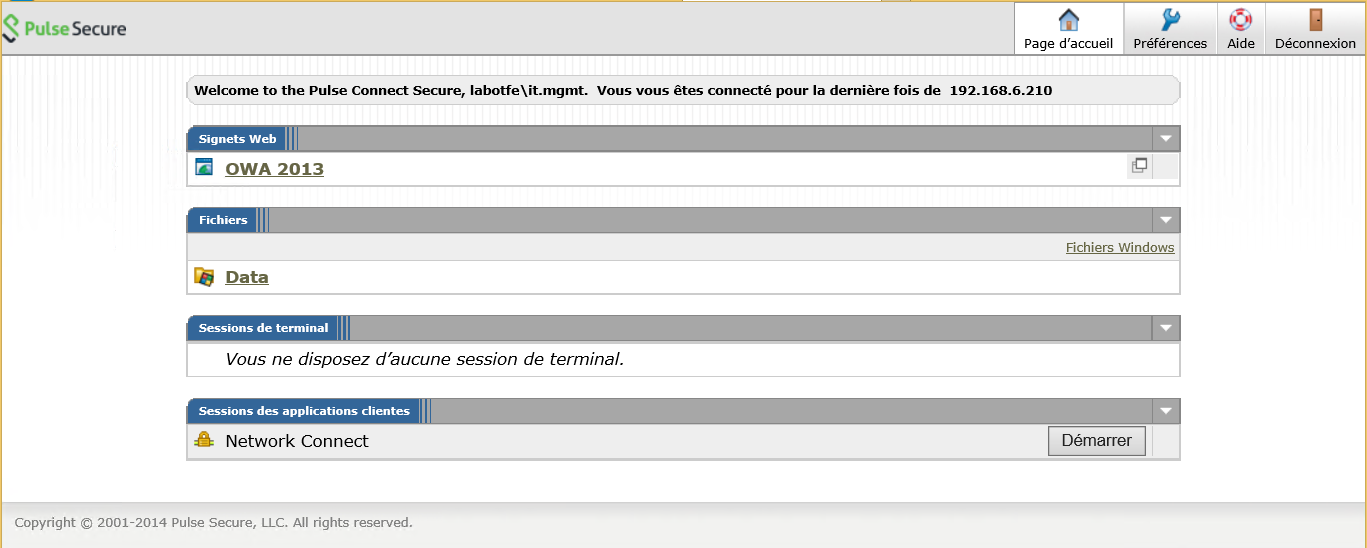
\includegraphics[width=16cm]{juniper/portail.png}
	\caption{\textit{Bookmarks} associés à un membre du groupe It Tech}
	\label{fig:bookmarks}
\end{figure}

\subsubsection{VPN - Pulse Secure}
Une fois le client installé, l'utilisateur saisit ses identifiants dans la fenêtre de Pulse Secure. 
La connexion se fait automatiquement. 
Pour une question de sécurité, la passerelle essaie d'établir une connexion en ESP et elle peut passer en SSL en cas d'échec de la connexion ESP.
L'ESP se fait en encapsulant les paquets dans un paquet UDP sur un port précis.
Mais si ce port est bloqué à un endroit entre le client et la passerelle, la connexion ESP est impossible.
L'option de fallback peut être désactivé pour améliorer la sécurité. 

Comme les utilisateurs ont un rôle assigné, on définit à chaque rôle un range d'adresse sur la passerelle pour les utilisateurs (voir Fig.\ref{fig:profilVPN} p.\pageref{fig:profilVPN}).
Ainsi le rôle "It Tech" possède les adresses du range 172.16.64.192/27 et le rôle "All Employee" les adresses du range 172.16.64.224/27.
De cette manière, on peut gérer les accès au niveau du firewall de façon granulaire, c'est-à-dire en autorisant seulement certaines adresses à accéder à certaines ressources.
\begin{figure}[ht]
	\centering
	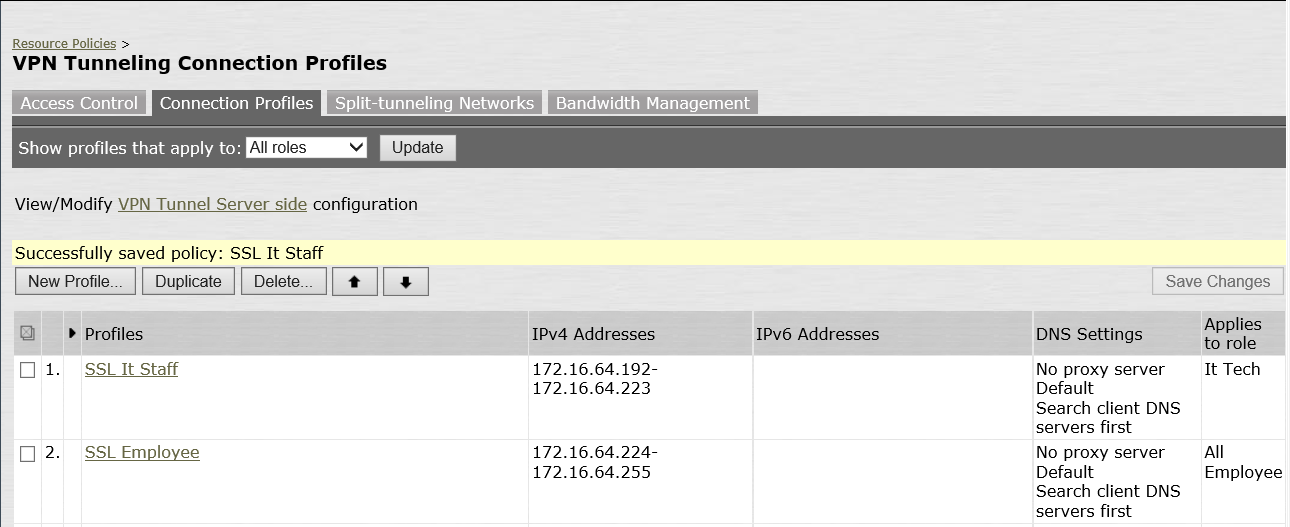
\includegraphics[width=16cm]{juniper/VPNProfiles.png}
	\caption{Profils VPN}
	\label{fig:profilVPN}
\end{figure}
\section{Solution Windows/DirectAccess}
\section{Solution Cisco/AnyConnect}
La solution Cisco diffère des autres solutions, car l'ASA\footnote{Adaptive Security Appliance} a des fonctions plus limitées.
Il n'offre que trois VLAN avec la licence de base, dont le troisième ne peut communiquer que dans un seul sens.

À l'instar de la solution Juniper, cette solution offre l'accès soit via un portail web, soit via un client VPN, AnyConnect.

\subsection{Schéma de l'infrastructure}
L'ASA fait office de pare-feu et de passerelle SSL voir Fig.\ref{fig:schemaCisco} p.\pageref{fig:schemaCisco}.
Comme chaque interface doit appartenir à un VLAN, l'un des VLAN est la zone \textit{outside} et l'autre est la zone \textit{inside}.
La zone \textit{outside} fait référence au réseau du laboratoire et l'\textit{inside} est mon domaine.
Dans ce cas-ci, les ordinateurs et les serveurs ne sont plus dans des zones distinctes (voir Fig.\ref{fig:schemaCisco} p.\pageref{fig:schemaCisco}).
\begin{figure}[ht]
	\centering
	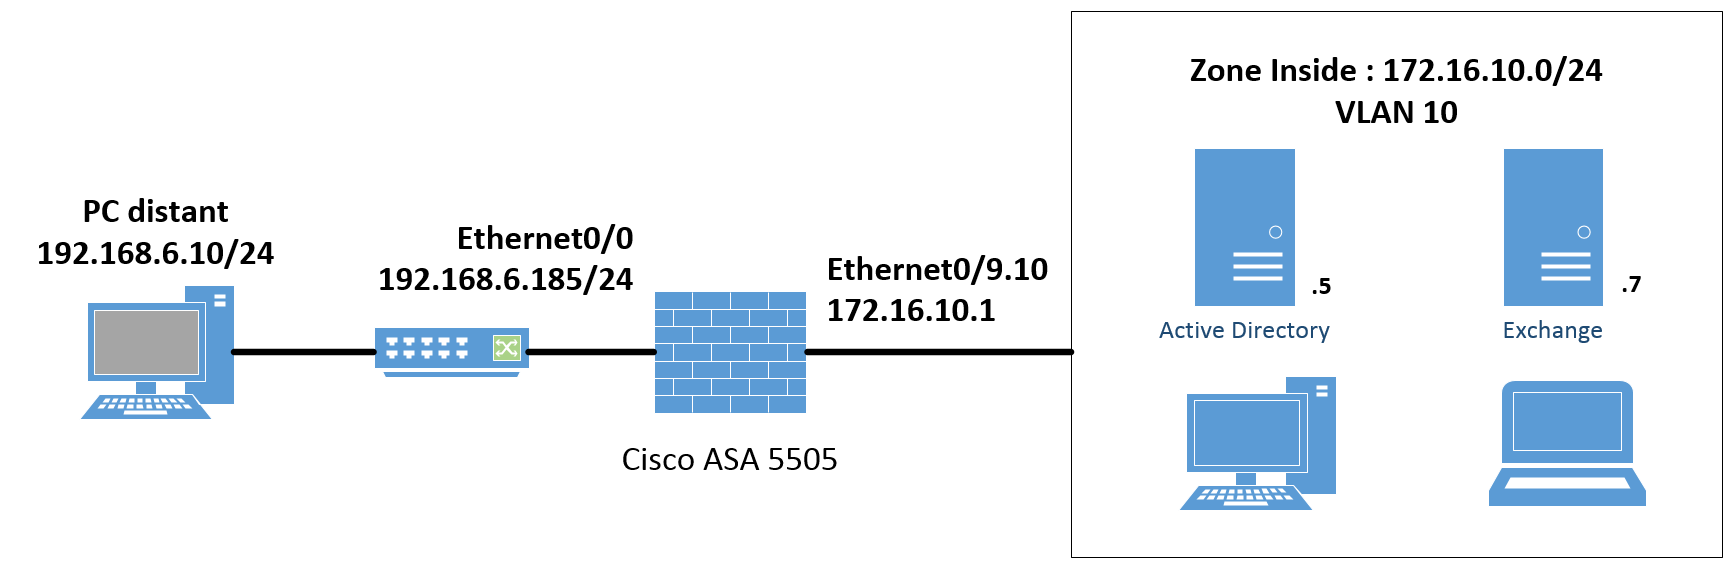
\includegraphics[width=16cm]{Cisco/schema.png}
	\caption{Adressage des interfaces}
	\label{fig:schemaCisco}
\end{figure}
Pour l'adressage, j'ai conservé le même plan sauf que mon ordinateur interne se retrouve avec une adresse 172.16.10.0/24 (voir Fig.\ref{fig:ifCisco} p.\pageref{fig:ifCisco}).
\begin{figure}[ht]
	\centering
	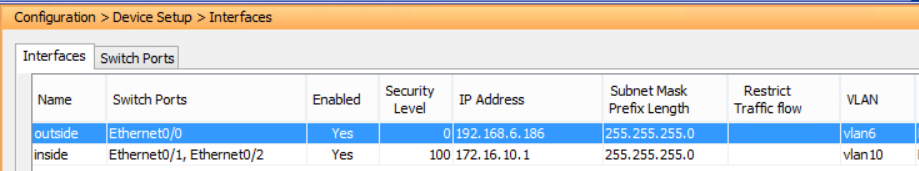
\includegraphics[width=16cm]{Cisco/interfaces.png}
	\caption{Adressage des interfaces}
	\label{fig:ifCisco}
\end{figure}

\subsection{Configuration de l'ASA}
Toute la gestion des connexions et des règles de pare-feu se fait via le même interface graphique, à savoir l'ASDM\footnote{Adaptive Security Device Manager}.
L'ASDM est à installer sur une machine cliente, qui possède Java.

Il est également possible de gérer l'ASA en ligne de commande, mais cette pratique n'est pas recommandée à moins de connaître toutes les commandes existantes.

\subsubsection{Gestion des accès}
L'authentification est vérifiée par l'Active Directory. 
Dans ce cas-ci, la configuration est moins simple, vu qu'il faut connaitre les attributs LDAP pour aller chercher dans les OU les utilisateurs et l'administrateur (voir Fig.\ref{fig:authCisco}p.\pageref{fig:authCisco}).
\begin{figure}[ht]
	\centering
	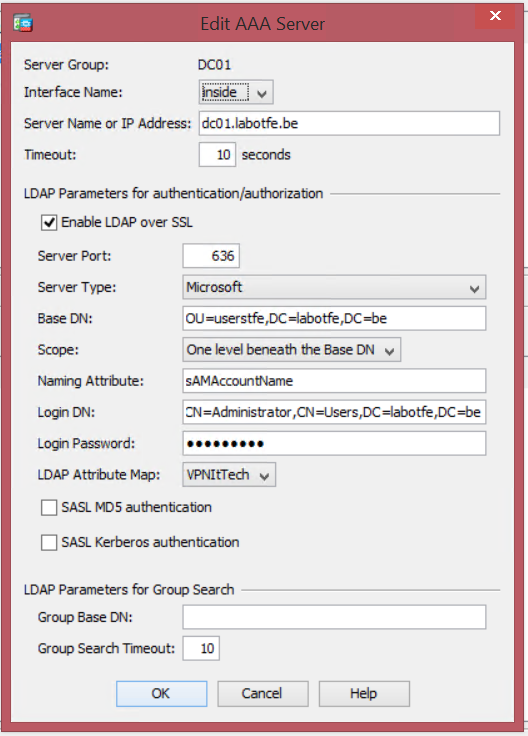
\includegraphics{Cisco/AAA-Ldap.png}
	\caption{Configuration de l'authentification des utilisateurs}
	\label{fig:authCisco}
\end{figure}

\subsubsection{VPN}
Tout d'abord, il faut créer le pool d'adresse pour les clients VPN.
En plus, il est intéressant d'associer des objets aux différents éléments de l'infrastructure pour faciliter la configuration (voir Fig.\ref{fig:objectCisco} p.\pageref{fig:objectCisco}).
\begin{figure}[ht]
	\centering
	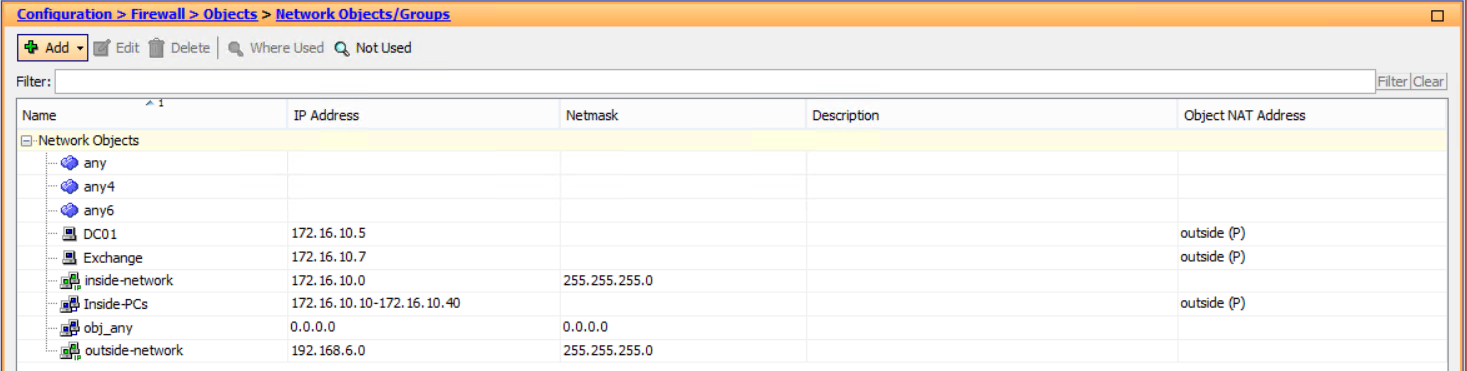
\includegraphics[width=16cm]{Cisco/objects.png}
	\caption{Configuration des objets}
	\label{fig:objectCisco}
\end{figure}

Ensuite, il faut initialiser le "Group Policy".
Ce groupe permet l'attribution des adresses, et aussi de plein de propriétés issues des groupes par défaut, car il hérite par défaut des propriétés de ces groupes. 
Comme on peut le voir sur la Fig.\ref{fig:gpCisco} p.\pageref{fig:gpCisco}, mon groupe \textit{VPNAccess} hérite de deux éléments, par contre pour l'adressage, il va chercher le pool que j'ai défini. 
\begin{figure}[ht]
	\centering
	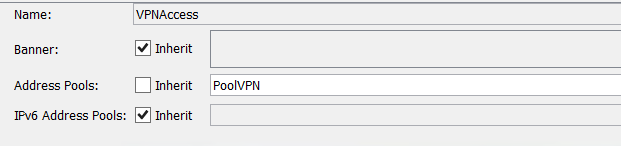
\includegraphics{Cisco/GroupPoliciesVPN.png}
	\caption{Configuration du groupe \textit{VPNAccess}}
	\label{fig:gpCisco}
\end{figure}

Finalement, il reste à configurer le profil de connexion voir Fig.\ref{fig:cpCisco} p.\pageref{fig:cpCisco}.
\begin{figure}[ht]
	\centering
	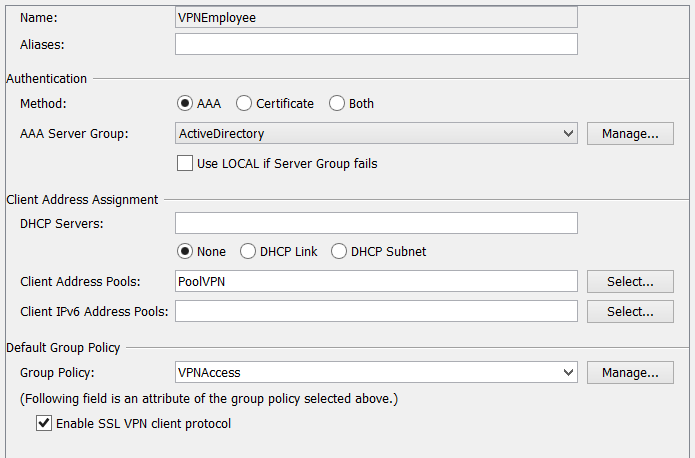
\includegraphics{Cisco/ConnectionProfile.png}
	\caption{Configuration du profil de connexion}
	\label{fig:cpCisco}
\end{figure} 
Il permet de définir le mode d'authentification, et le groupe à associer aux clients.
Particularité, il faut préciser le pool d'adresse même si cette information est déjà donnée dans le groupe associé.

\chapter{Scénario de test}
\section{Scénario de test}
Le but de ce travail est de tester les accès distants aux ressources d'une entreprise.
Dans les points précédents, j'ai décrit l'ensemble des ressources et des méthodes d'accès.

Dans ce chapitre, j'explique le scénario de test pour comparer les solutions d'accès sur des points similaires.

La première ressource à contacter est le serveur mail de l'entreprise. 
Pour ce faire, Outlook est installé sur la machine distante. 
Il est configuré pour se connecter à la boîte mail de \textit{it.mgmt@labotfe.be}.

Les fichiers sont la deuxième ressource à accéder.
Un disque mappé est configuré par GPO aux utilisateurs du domaine. 

La troisième ressource est l'intranet de l'entreprise.
Cet intranet est composé d'une seule page web, qui affiche un message de bienvenue.

\chapter{Critères de comparaison}
Les critères de comparaison vont permettre de classer les différentes solutions.
Les critères sélectionnés sont de plusieurs types.
Il y a des critères liés aux tests de connectivité, d'autres sont liés aux fonctionnalités ou aux technologies utilisées.

\section{Les critères sélectionnés}
Il existe un nombre importants de critères pour réaliser ce comparatif.
J'ai décidé d'en choisir seize qui montrent bien les différences entre les différentes solutions sélectionnées. 
Mes choix se sont portés sur d'une part des tests de connectivité, vu que l'un des objectifs essentiels des VPNs est l'accès aux ressources.
D'autre part, ils portent sur les suites de chiffrement et les protocoles supportés.
Un autre objectif des VPN est la sécurisation des données. 
De plus, un critère plus personnel sur l'utilisation des systèmes est intéressante.
Car n'ayant aucune expérience avec ce genre de systèmes, j'ai dû apprendre à les utiliser.
Finalement, un critère financier est important à signaler.
\rowcolors{2}{lightgray}{}
\begin{longtable}{p{4cm}|p{12cm}}
	\toprule
	\textbf{Critère} & \textbf{Description} \endhead
    \hline 
    Connexion Outlook & Test de connectivité entre le client mail Outlook et le serveur Exchange \\
    \hline
    Connexion Outlook Web App & Test de connectivité entre la machine cliente et la Web App du serveur Exchange. Dans ce cas, l'OWA n'est accessible que depuis le réseau interne, il faut donc que les machines distantes aient un accès au réseau interne.\\
    \hline
    Connexion au DFS Namespace & Test de connectivité entre la machine cliente et le DFS Namespace \\
    \hline
    Connexion à l'intranet & Test de connectivité entre la machine cliente et le serveur Web interne, qui héberge l'intranet \\
    \hline
    Type de tunnel & La connexion se fait par un tunnel VPN, mais quel type de tunnel ?. Les réponses possibles sont SSL ou ESP/IPSec.\\
    \hline
    Algorithme de chiffrement par défaut & Lors de la configuration, un algorithme ou un ensemble d'algorithme est sélectionné par défaut.\\
    \hline
    Version de SSL/TLS par défaut & Il existe plusieurs versions de ces protocoles. Le but est de savoir le(s)quelle(s) a/ont été sélectionné par défaut.\\
    \hline
    Algorithme de chiffrement offrant le plus de sécurité & Lors de la configuration, il est possible de sélectionner le(s) algorithme(s) souhaité(s). Ce critère met en lumière l'algorithme le plus sécurisé supporté par le système.\\
    \hline
    Version de SSL/TLS maximum supportée & Le but est de savoir qu'elle est la version maximale de la technologie qui est supportée par le système.\\
    \hline
    Facilité de configuration & Ce critère est plus personnel, mais il se base sur un code que j'explique plus tard.\\
    \hline
    Fallback SSL & Ce test vérifie la présence d'une option pour le passage de IPSec vers SSL en cas de problème lors de la connexion en IPSec.\\
    \hline
    Host Checker & Ce test signale la présence d'une méthode pour vérifier que l'hôte peut se connecter en VPN.\\
    \hline
    Méthode d'authentification & Ce test précise le mode d'authentification utilisé lors des tests, ainsi que les autres méthodes d'authentification supportées.\\
    \hline
    Split Tunneling & Signale la présence ou non de l'option. Si oui, le fonctionnement par défaut.\\
    \hline
    Push Mail & Ce test porte sur l'utilisation d'ActiveSync pour le push mail.\\
    \hline
    Prix & Le prix tient compte du prix des appareils nécessaires à la réalisation de l'infrastructure.\\
    \bottomrule
    \caption{Critères de comparaison}
	\label{tab:criteres}\\
\end{longtable}

\subsection{Explication du critère "Facilité de configuration"}
Ce critère est plus personnel, mais il se base sur les points suivants.
J'attribue une note entre 1 et 5 sur la configuration et une note entre 1 et 5 sur l'interface graphique.

Pour la configuration, la note de 5 signifie qu'elle est simple.
C'est-à-dire que le guide d'administration suffit largement pour configurer les différents éléments à mettre en place.
Par contre, une note de 1 signifie que la configuration n'est pas simple.
Il faut chercher plus loin que le guide d'administration fourni, voir demander sur des forums pour trouver la bonne marche à suivre.

Pour l'interface graphique, une note de 5 signifie que l'interface est intuitive. 
Il est relativement aisé de trouver les éléments à modifier, les menus sont bien présentés.
À l'inverse, une note de 1 montre que l'interface est mal conçue.

\section{Grille de comparaison}
Sur base des critères et des différentes architectures/solutions, j'ai dressé un tableau de comparaison de ces différentes solutions.

\begin{tabular}{m{4cm}m{12cm}}
\ok & La connexion est établie / présence de l'option \\
\nok & La connexion n'est pas établie / option non disponible \\
\unk & L'information n'est pas disponible \\
N/A & Le test ne s'applique pas à cette solution \\
\end{tabular}

\begin{landscape}
\begin{longtable}{>{\centering\columncolor{lightgray}}m{4cm}|>{\centering}m{3.3cm}|>{\centering}m{3.3cm}|>{\centering}m{3.3cm}|>{\centering}m{3.3cm}|m{3.3cm}<{\centering}}
	\toprule
	\textbf{Critère} & \textbf{Juniper - Portail Web} & \textbf{Juniper - Pulse Secure} & \textbf{Cisco Clientless} & \textbf{Cisco AnyConnect} & \textbf{DirectAccess} \endhead
    \hline
    Connexion Outlook & N/A & \ok & N/A & \ok & \ok \tabularnewline
    \hline
    Connexion Outlook Web App & \ok & \ok & \ok & \ok & \ok \tabularnewline
    \hline
    Connexion au DFS Namespace & \ok & \ok & \nok & \ok & \ok \tabularnewline
    \hline
    Connexion à l'intranet & \ok & \ok & \ok & \ok & \ok \tabularnewline
    \hline
    Type de tunnel & SSL & ESP & SSL & DTLS & IPSec \tabularnewline
    \hline
    Algorithme de chiffrement par défaut & 128bit et + & AES128/SHA1 & AES256-128-RC4-3DES/SHA1 & RSA-AES128/SHA1 & AES-CBC-128/SHA-256 \tabularnewline
    \hline
    Version de SSL/TLS par défaut & SSLv3 \& TLS & SSLv3 \& TLS & SSLv2, SSLv3 et TLSv1 & SSLv2, SSLv3 et TLSv1 & \unk \tabularnewline
    \hline
    Algorithme de chiffrement offrant le plus de sécurité & 168bit et + & AES256/SHA1 & AES256/SHA1 & AES256/SHA1 & TLS-ECDHE-RSA-AES256-CBC-SHA384 \tabularnewline
    \hline
    Version de SSL/TLS maximum supportée & TLSv1 & TLSv1 & TLSv1 & TLSv1 & \unk \tabularnewline
    \hline
    Facilité de configuration & 10 & 10 & 6 & 2 & 8 \tabularnewline
    \hline
    Fallback SSL & N/A & \ok (option) & N/A & \nok & N/A \tabularnewline
    \hline
    Host Checker & \ok & \ok & \ok & \ok & \ok \tabularnewline
    \hline
    Méthode d'authentification & Active Directory & Active Directory & Active Directory & Active Directory & Kerberos \tabularnewline
    \hline
    Split Tunneling & N/A & \ok (désactivé) & N/A & \ok (activé) & \ok (activé) \tabularnewline
    \hline
    Push Mail & \multicolumn{2}{c|}{\ok} & \unk & \unk & N/A \tabularnewline
    \hline
    Prix (en euro) & \multicolumn{2}{c|}{5400} & \multicolumn{2}{c|}{500-1000} & 4200 \tabularnewline
    \bottomrule
    \caption{Tableau de comparaison}
	\label{tab:comparaison}\\
\end{longtable}
\end{landscape}
\subsection{Commentaires}
\subsubsection{Solution Juniper}
La solution Juniper est la meilleure des solutions, vu qu'elle offre toute les fonctionnalités demandées, ainsi qu'une interface graphique intuitive. 
Le guide d'administration est suffisamment complet que pour réaliser la configuration de manière autonome.

La seule remarque à faire porte sur l'utilisation d'ActiveSync pour le push mail.
Lors des tests, j'employais un utilisateur, qui est administrateur du domaine.
Par défaut, le serveur Exchange n'autorise pas les administrateurs à utiliser ActiveSync.
Pour éviter de modifier les paramètres de cet utilisateur, j'ai pris un utilisateur standard pour mes tests.

\subsubsection{Solution Windows}
La solution Windows DirectAccess a son intérêt, mais elle est plus limitée.
Elle ne s'appuie que sur l'utilisation de système d'exploitation Windows.
Elle n'est pas compatible avec les appareils de type smartphone, ce qui réduit un peu l'utilité de ce service pour accéder au mail depuis l'extérieur.
Le critère "Host Checker" est sous-entendu valide, car DirectAccess est déployé via une GPO liée à un groupe de sécurité.
Donc, les machines utilisant DirectAccess sont vérifiées par l'administrateur réseaux, car il a dû placer les ordinateurs concernés dans le groupe de sécurité.

Il n'est pas possible de déterminer avec précisions quels sont les algorithmes de chiffrement utilisés par DirectAccess.
Une liste des algorithmes supportés est disponible sur l'Internet\footnote{\url{http://directaccess.richardhicks.com/2014/09/23/directaccess-ip-https-ssl-and-tls-insecure-cipher-suites/}}.
Sur cette liste, on remarque que des algorithmes sans chiffrement sont utilisables.
Néanmoins, ces algorithmes sont utilisés par IP-HTTPS.
Les paquets entre le client et le serveur sont chiffrés par IPSec, il n'est donc pas utile de chiffrer une deuxième fois les paquets.

\subsubsection{Solution Cisco}
La solution Cisco est sans doute la moins agréable à utiliser.
Les problèmes de version du logiciel sont pour le moins dérangeantes.
Pour des raisons techniques, j'ai dû travailler avec la version 8.3 du logiciel.
À la base, la version 9.3 était prévue.
Mais l'ASA ne disposant que de \numprint[MB]{256}, il m'était impossible de désarchiver le package AnyConnect nécessaire au déploiement du client sur les machines.
En cherchant sur le site de Cisco, la dernière version compatible avec l'ASA mis à disposition est la version 8.3.
Malheureusement, cette version ne gère pas bien les certificats.
J'ai donc désactivé l'authentification de l'ASA via le certificat.

De plus, en passant en version 8.3, la connexion au serveur de fichier n'est plus possible.
Avec la version 9.3, il était possible d'accèder au DFS Namespace.

Par ailleurs, la solution Cisco impose l'utilisation de Java.
Car l'ASDM et les services accessibles via le portail web se base sur Java pour fonctionner.

\subsection{Les prix des solutions}
Les trois solutions décrites ont des prix largement différents, car les techniques de ventes varient d'un fabricant à l'autre.

La solution Juniper est la plus chère avec un prix minimum de \euro{5400}.
Ce prix comprend la passerelle, plus une licence pour dix utilisateurs et le support de trois ans.

La solution Cisco est la moins chère avec un prix entre \euro{500} et \euro{1000}.
Le prix communiqué comprend le firewall avec la licence de base.

La solution Windows est entre les deux.
Son prix est plus variable selon le serveur choisi, mais la licence Windows Server coûte à elle seul \euro{1200}.
Un serveur de puissance correcte coûte dans les \euro{3000}.




\chapter*{Conclusion}
\addcontentsline{toc}{chapter}{Conclusion}
Ce rapport abouti à la réalisation d'un comparatif des solutions d'accès distant.
Ce comparatif met en évidence les différences de philosophies de la part des fabricants.
En effet, chaque solution possède ses propres caractéristiques et fonctionnalités.
Même si les fonctionnalités sont similaires, les implémentations diffèrent.\\

Mes recommandations sont les suivantes.

La solution Juniper est de loin, la plus agréable à utiliser.
Elle offre une interface claire, et la configuration est aisée même pour un débutant.

Le guide d'administration est complet et clair.
Par contre, c'est la solution la plus chère.
À éviter pour des petits budgets.\\

La solution Windows est sans doute la plus simple à configurer, mais son fonctionnement peut être une source de vulnérabilité.
En effet, la procédure de connexion étant automatique, l'utilisateur n'a pas de possibilité d'empêcher l'établissement de la connexion entre son ordinateur et le réseau de l'entreprise.
Néanmoins, il a la possibilité de couper la connexion une fois qu'elle est établie.
Le configuration est simple du fait qu'elle est automatisée.

Par contre, le guide en ligne fourni par Microsoft n'est pas clair.
Il détaille plusieurs types d'installation, il n'est donc pas évident de trouver celle qui s'applique à son propre cas.\\

Le solution Cisco est celle à éviter.
L'interface n'est pas intuitive.
Pour qu'un changement soit effectif, il est nécessaire de passer par plusieurs fenêtres.
Des groupes par défaut viennent polluer l'interface, car ils ne sont pas supprimables.
Les groupes qui sont créés par l'administrateur héritent de toutes les propriétés du groupe par défaut.
Il est donc nécessaire soit d'activer le groupe par défaut, soit de modifier tous les champs du nouveau groupe, ce qui alourdi la tâche de l'administrateur.

Les problèmes de version sont aussi un désavantage dans ce cas.
Car ce qui marche dans une version ne marche plus dans une autre.

De plus, le guide d'administration n'est pas clair.
Il est complet, mais les informations fournies ne sont pas assez approfondies pour comprendre l'ensemble des réglages.
 
\input{Bibliographie}
\end{document}